\begin{boxC}
% قسمت الف :
\begin{itemize}
    \item 
    به این دلیل که داده‌های ما باید حداقل دارای یک 
    \lr{Relevant Query}
    باشند.
    و یا حداقل باید از سایر تکنیک‌ها برای پیش‌پردازش متن استفاده شود.

    مانند حذف کلمات بسیار پرتکرار و یا همان به اصطلاح مرسوم 
    \lr{Stop Words}.

    و همچنین یکسان کردن کلمات هم‌خانواده 
    \lr{Stemming}

    اما همانطور که قبل‌تر ذکرشد ، مساله اصلی ما ایجاد و به عبارت بهتر پیش‌بینی 
    \lr{Relevant Query}
    می‌باشد.

    به ازای هر داکیومنت ، یا به عبارتی شفاف‌تر در حوزه کتاب باید به ازای هر پاراگراف ، فصل ، نیم بند ، بخش و یا هر
    دسته‌بندی دیگری باید یک کوئری مرتبط داشته‌باشیم.

    مهمترین چالش‌پیش رو اولیه این می‌تواند باشد.

    جلوتر به چگونگی ایجاد و یا پیش‌بینی کوئری مرتبط با سند می‌پردازیم.



    \item 
    برای آموزش دادن به مدل برای اسناد با حجم داده زیاد ابتدا بایستی از تکنیک‌های پیش پردازش متن استفاده کنیم.
    
    (\lr{Preprocessing Techniques})

    در زیر به چند تکنیک از این روش خواهیم پرداخت :

    \begin{enumerate}
        \item 
        \lr{Query Reformulation}
        
        \item 
        \lr{doc2query}

        \item 
        \lr{DeepCT}

        \item 
        \lr{DeepImpact(Combine doc2query with DeepCT)}
    \end{enumerate}


    \item 
    قبل از هرکاری می‌بایستی که عملیات پیش‌پردازش بر روی اسناد انجام شود.
    گسترش هر داکیومنت با پیش‌بینی کوئری مرتبط آن با مدل‌های 
    \lr{Transformer}
    صورت خواهدگرفت.
    (مانند \lr{Seq2Seq})
    
    ساختن یک مدل زبانی بزرگ شامل موارد زیر است :
    \begin{enumerate}
        \item 
        مجموعه داده (جمع‌آوری و تهیه یک مجموعه داده وسیع از کتب و منابع مرتبط)

        \item 
        مدل زبانی
        (استفاده از مدل زبانی بزرگ بر اساس شبکه‌های عصبی )

        \item 
        ماژول پرسش و پاسخ
        (ایجاد یک ماژول پرسش و پاسخ که وظیفه پردازش سوالات کاربر را برعهده دارد.
        )

        
        \item 
        مدیریت دانش
        (در واقع ایجاد یک نوع ایندکس بر روی متون کتاب‌ها بر اساس موضوعات و مفاهیم مختلف)

        \item 
        بهبود پرسش و پاسخ
        (ارزیابی پاسخ‌های تولیدشده بر اساس برخی معیارهای ارزیابی)
        
    \end{enumerate}
    
\end{itemize}
    
\end{boxC}

\begin{figure}[h]
        \centering
        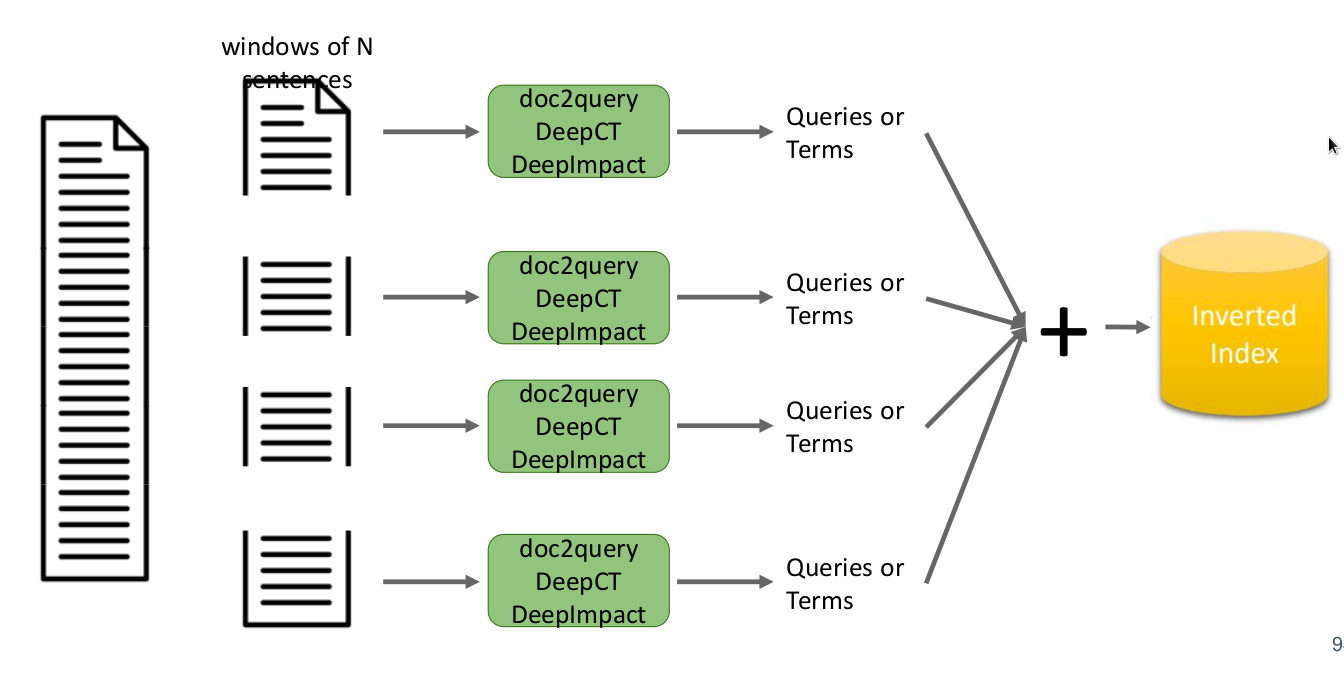
\includegraphics
        [width = 0.8\textwidth]
        {IR4/images/2-1.png}
        \caption{نمایی از عملیات پیش‌پردازش بر روی متون بزرگ}
        \label{fig:enter-label}
\end{figure}

\begin{figure}[h]
    \centering
    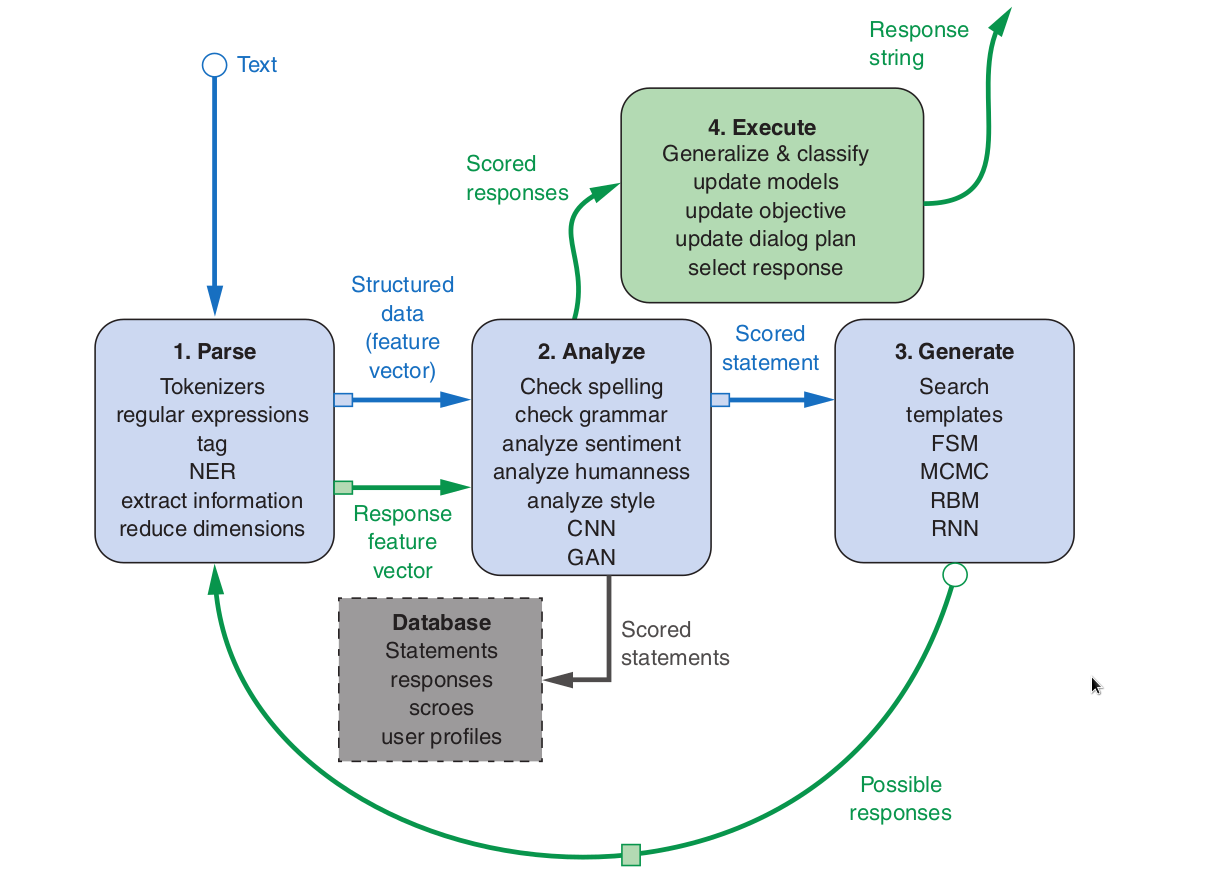
\includegraphics
    [width = 0.8\textwidth]
    {IR4/images/chatbot_pipeline.png}
     \caption{معماری یک سیستم مدل زبانی بزرگ ساده}
    % \caption{Caption}
    \label{fig:enter-label}
\end{figure}